\tikzset{fontscale/.style = {font=\relsize{#1}}
    }
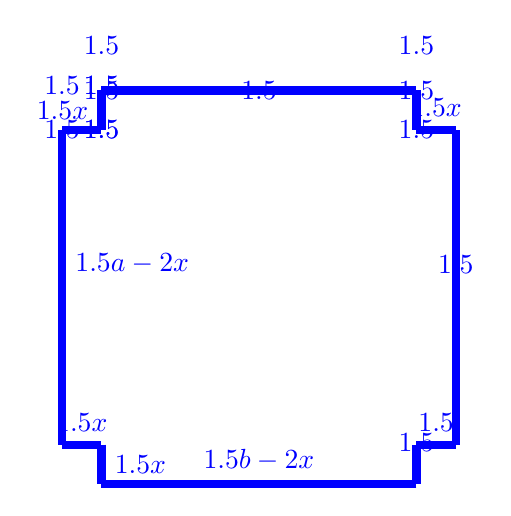
\begin{tikzpicture}[scale=1,blue,
fontscale=1.5,
line width=3pt,
         dot/.style = {
     fill = black!30!brown,
      circle,
      inner sep =2pt,
      minimum size = 4pt
    }
  ]
%%%%%%%%%%%%%%%%%%%%%%%%%%%%%%%%%%%%%%
 %\draw [very thin, style=gray!50, step=0.5] (-3,-2) grid (3,2);
% \draw [thin, gray!60] (0,0) grid (6,6);
\coordinate (O) at (0,0);
\coordinate (A) at (0,4.5);
\coordinate (B) at (0.5,4.5);
\coordinate (C) at (0.5,5);
\coordinate (D) at (4.5,5.0);
\coordinate (F) at (5,4.5);
\coordinate (E) at (4.5,4.50);
\coordinate (G) at (5,0.5);
\coordinate (H) at (4.5,0.5);
\coordinate (I) at (4.5,0);
\coordinate (J) at (0.5,0);
\coordinate (K) at (0.5,0.5);
\coordinate (L) at (0,0.5);
\draw[]           (A)node[
                               label = {}]{}-- (B) node[
                               label = {}] {};
\draw[color=blue]           (B)node[
                               label = {}]{}-- (C) node[
                               midway, left ] {$x$};
% \draw[blue,ultra thick] (1,0) arc (0:90:1); 
\draw[color=blue]           (C)node[
                               label = {}]{}-- (D) node[
                                midway] {};
\draw          (D)node[
                               label = {}] {} -- (E) node[
                                 ] {};
\draw          (E)-- (F) node[midway,above
                             ] {$x$};
\draw          (G)-- (F) node[midway,above
                             ] {};
\draw          (G)-- (H) node[midway,above
                             ] {};
\draw           (I)-- (H) node[midway,above
                             ] {};
\draw           (I)-- (J) node[midway,above
                             ] {$b-2x$};
\draw          (K)-- (J) node[midway, right
                             ] {$x$};
\draw          (K)-- (L) node[midway,above 
                             ] {$x$};
\draw          (A)-- (L) node[midway,above right 
                             ] {$a-2x$};
%  \draw[color=blue] (-0.1,0.1) node {\small $O$};
%  \draw[color=blue] (-0.1,0.82) node {$t$};
% \draw[color=blue] (0.97,0.88) node {\small $P=(s,t)$};
% \draw[color=blue] (0.6,-0.1) node {$s$};
  \end{tikzpicture}
